%=======================02-713 LaTeX template, following the 15-210 template==================
%
% You don't need to use LaTeX or this template, but you must turn your homework in as
% a typeset PDF somehow.
%
% How to use:
%    1. Update your information in section "A" below
%    2. Write your answers in section "B" below. Precede answers for all 
%       parts of a question with the command "\question{n}{desc}" where n is
%       the question number and "desc" is a short, one-line description of 
%       the problem. There is no need to restate the problem.
%    3. If a question has multiple parts, precede the answer to part x with the
%       command "\part{x}".
%    4. If a problem asks you to design an algorithm, use the commands
%       \algorithm, \correctness, \runtime to precede your discussion of the 
%       description of the algorithm, its correctness, and its running time, respectively.
%    5. You can include graphics by using the command \includegraphics{FILENAME}
%
\documentclass[11pt]{article}
\usepackage{amsmath,amssymb,amsthm}
\usepackage{tikz}
\usetikzlibrary{arrows,positioning, calc, matrix}
\tikzstyle{vertex}=[draw,fill=black!15,circle,minimum size=20pt,inner sep=0pt]
\usepackage{graphicx}
\usepackage[margin=1in]{geometry}
\usepackage{fancyhdr}
\usepackage{mathtools}
\usepackage{placeins}
\usepackage{listings}
\usepackage{color}
\usepackage{forest}
\usepackage{tikz}
\usepackage{caption}
\usepackage{mathtools}
\DeclarePairedDelimiter{\ceil}{\lceil}{\rceil}
\DeclarePairedDelimiter{\floor}{\lfloor}{\rfloor}

\definecolor{dkgreen}{rgb}{0,0.6,0}
\definecolor{gray}{rgb}{0.5,0.5,0.5}
\definecolor{mauve}{rgb}{0.58,0,0.82}

\lstset{frame=none,
  language=Java,
  aboveskip=3mm,
  belowskip=3mm,
  showstringspaces=false,
  columns=flexible,
  basicstyle={\small\ttfamily},
  numbers=none,
  numberstyle=\tiny\color{gray},
  keywordstyle=\color{blue},
  commentstyle=\color{dkgreen},
  stringstyle=\color{mauve},
  breaklines=true,
  breakatwhitespace=true,
  tabsize=3
}

\setlength{\parindent}{0pt}
\setlength{\parskip}{5pt plus 1pt}
\setlength{\headheight}{13.6pt}
\newcommand\question[2]{\vspace{.25in}\hrule\textbf{#1 #2}\vspace{.5em}\hrule\vspace{.10in}}
\renewcommand\part[1]{\vspace{.10in}\textbf{(#1)}}
\newcommand\algorithm{\vspace{.10in}\textbf{Algorithm: }}
\newcommand\correctness{\vspace{.10in}\textbf{Correctness: }}
\newcommand\runtime{\vspace{.10in}\textbf{Running time: }}
\pagestyle{fancyplain}
\lhead{\textbf{\NAME}}
\chead{\textbf{HW\HWNUM}}
\rhead{\today}
\begin{document}\raggedright
%Section A==============Change the values below to match your information==================
\newcommand\NAME{Sean Connor (443-414-5111)}  % your name
\newcommand\HWNUM{ PA3}              % the homework number
%Section B==============Put your answers to the questions below here=======================
\question{Analysis}{}
\part{a} 
Initially, I had created a ``greedy'' algorithm. The pseudocode for this is below.
\begin{lstlisting}
/* Java/pseudocode for ``greedy'' interleaving algorithm */
int i = 0;
int j = 0;
for (item : s) {
	if (item == x[i]) {
		increment(i);
	}
	else if (item == y[j]) {
		increment(j);
	}
	else {
		return false;
	}
}
return true;
\end{lstlisting}
In this algorithm, the increment() method performs i++/j++ if i/j is not the last character of x/y. If i/j is last character of x/y, then reset i/j to zero. In some cases, this algorithm produces the correct result and runs in O(n) time - for example, in the case given by the prompt. However, a simple example reveals that it does not always produce the correct solution. For example, consider the case where $x=00$, $y=01$, and $s=01$. The above algorithm would return \textit{false} when it is clear that $s$ is in fact an interleaving of $x$ and $y$. Clearly, a better solution is required.

Thinking back to recent topics covered in class, it was evident that this is an ideal problem for a bottom-up dynamic programming algorithm. In this case, if $s$ is an interleaving of $x$ and $y$, then any subproblem of $s$ is also an interleaving of $x$ and $y$. Thus, the simplest algorithm that produces the correct result simply iterates through an s.length by s.length array and calculates subproblems of increasing size until reaching the maximum problem size (occurs when, given a solution array a[i][j], $i+j=s.length$). An example of this is shown in Figure 1, and the Java/pseudocode is provided below. Because $s$ can be an interleaving of \textit{repeats} of $x$ and $y$, and  this could possibly be given where $s$ is simply a repeat of only $x$ or only $y$, it is neccesary to ``extend'' $x$ and $y$ to be the same length as $s$.

\begin{lstlisting}
/* Java/pseudocode for dynamic programming interleaving algorithm */
// Extend x and y to s.length (e.g. x=101 and s.length=7 --> extend(x) = 1011011)
x = extend(x);
y = extend(y);

// Create a 2D boolean array to store solution to the subproblems
boolean[][] a = new boolean[lenS+1][lenS+1];

// Nested for-loops to evaluate all subproblems
for (int i = 0; i <= s.length; i++) {
	for (int j = 0; j <= s.length; j++) {
		// This ensures only the the upper left diagonal is evaluates (i+j <= s.length)
		if (i + j <= s.length) {
			// This evaluates the top left square
			if (i == 0 AND j == 0){
				a[i][j] = true;
			} 
			// This evaluates the top row
			else if (i == 0) {
				a[i][j] = a[i][j-1] AND (y.charAt(j-1) == s.charAt(i+j-1));
			} 
			// This evaluates the left column
			else if (j == 0) {
				a[i][j] = a[i-1][j] AND (x.charAt(i-1) == s.charAt(i+j-1));
			} 
			// This evaluates everything else
			else {
				a[i][j] = (a[i][j-1] AND (y.charAt(j-1) == s.charAt(i+j-1))) OR
				           (a[i-1][j] AND (x.charAt(i-1) == s.charAt(i+j-1)));
			}
		}
	}
}
\end{lstlisting}

\begin{figure}[htbp!]
\centering
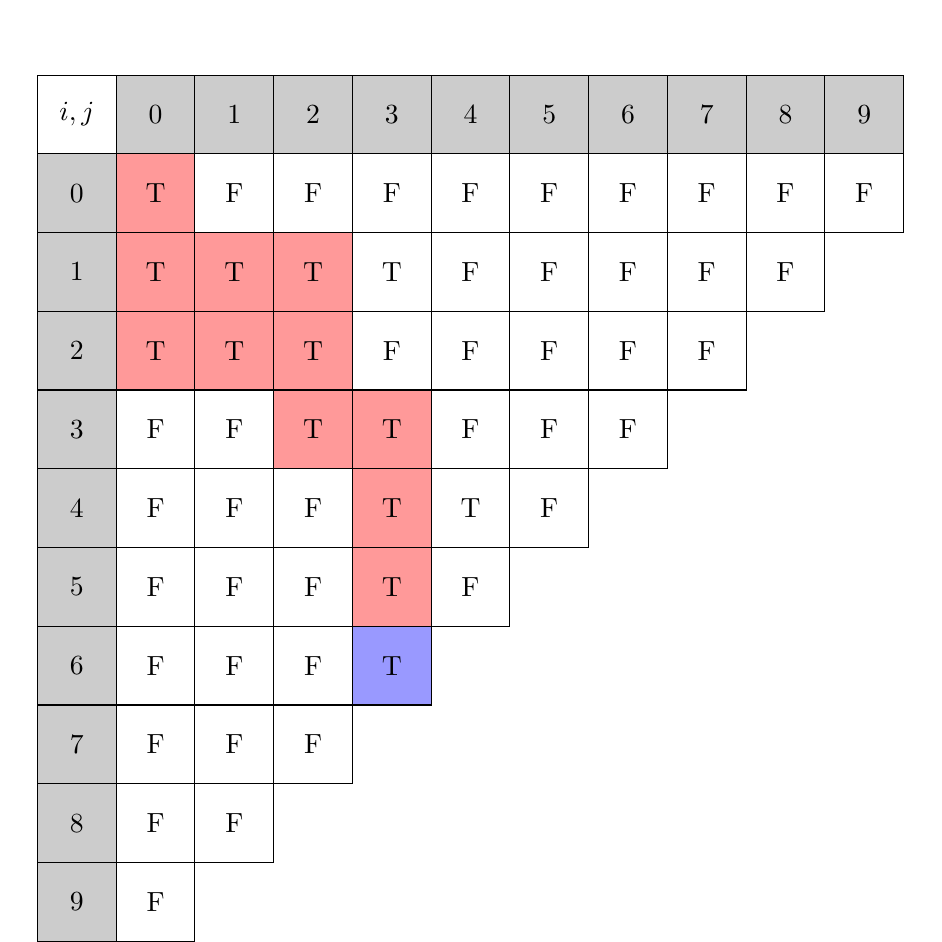
\begin{tikzpicture}
\tikzset{square matrix/.style={
    matrix of nodes,
    column sep=-\pgflinewidth, row sep=-\pgflinewidth,
    nodes={draw,
      minimum height=#1,
      anchor=center,
      text width=#1,
      align=center,
      inner sep=0pt
    },
  },
  square matrix/.default=1.0cm
}

\matrix[square matrix]
{
$i,j$ & |[fill=black!20]|0 & |[fill=black!20]|1 & |[fill=black!20]|2 & |[fill=black!20]|3 & |[fill=black!20]|4 & |[fill=black!20]|5 & |[fill=black!20]|6 & |[fill=black!20]|7 & |[fill=black!20]|8 & |[fill=black!20]|9 \\
|[fill=black!20]|0 & |[fill=red!40]| T & F & F & F & F & F & F & F & F & F \\
|[fill=black!20]|1 & |[fill=red!40]| T & |[fill=red!40]| T & |[fill=red!40]| T & T & F & F & F & F & F \\
|[fill=black!20]|2 & |[fill=red!40]| T & |[fill=red!40]| T & |[fill=red!40]| T & F & F & F & F & F  \\
|[fill=black!20]|3 & F & F & |[fill=red!40]| T & |[fill=red!40]| T & F & F & F \\
|[fill=black!20]|4 & F & F & F & |[fill=red!40]| T & T & F \\
|[fill=black!20]|5 & F & F & F & |[fill=red!40]| T & F \\
|[fill=black!20]|6 & F & F & F & |[fill=blue!40]| T \\
|[fill=black!20]|7 & F & F & F \\
|[fill=black!20]|8 & F & F \\
|[fill=black!20]|9 & F \\
};

\end{tikzpicture}
\caption{The example from the prompt (x=101, y=00, s=100010101). The subproblems are solved first, starting at $(0,0)$ which is always true. Squares colored in red indicate the possible ``path'' to the solution, and the square colored in blue indicates that $s$ is an interleaving of $x$ and $y$. Squares colored in grey represent the indices. A square can only be evaluated as true if either square to the left or above is also true \textit{and} if the character matches in $s$.}
\end{figure}

From the pseudocode provided above, it is clear that the algorithm runs in $O(n^2)$ time, where n is the length of the string s. Accessing array elements and the charAt() function are both constant-time ($O(1)$), and so the net complexity of this dynamic programming algorithm for determining whether a binary string $s$ is an interleaving of two other binary strings $x$ and $y$ is $O(n^2)$.

\part{b}
See code included in the src folder of zip file for algorithm implementation. Run time was evaluated by generating randomized test files. Ten each of the following were created and evaluated (numbers indicate string length):
\begin{itemize}
\item $x=y=5$ AND $s=20$
\item $x=y=10$ AND $s=100$
\item $x=y=100$ AND $s=1000$
\end{itemize}
In my code I did include a counter that incremented each time a comparison was made. However, comparisons were only included for the if-else if-else statements, and not the logical comparisons within each statement. Thus, the final tally will be off by some constant value. Regardless, the time complexity is the same $O(n^2)$.

The number of comparisons made per run is provided in each output file. The results are summarized here.
\begin{itemize}
\item $x=y=5$ AND $s=20$ $\longrightarrow$ \# comparisons = 902
\item $x=y=10$ AND $s=100$ $\longrightarrow$ \# comparisons = 20502
\item $x=y=100$ AND $s=1000$ $\longrightarrow$ \# comparisons = 2005002
\end{itemize}

From this, we can see that the time complexity is indeed $O(n^2)$ (see Figure 2). Thus, we have used dynamic programming to create an algorithm at efficiently and \textit{correctly} determines whether or not $s$ is an interleaving of $x$ and $y$. In addition, it is worth noting that creating test cases for this is quite tricky. Of the thirty randomized binary strings tested, none of them were interleavings.

\begin{figure}[!htbp]
  \includegraphics[width=\linewidth]{Untitled.png}
  \caption{The counted number of comparisons for each s.length.}
\end{figure}

\end{document}









